\item O sistema consiste de um disco $A$, de \SI{10}{\kilogram}, uma barra fina, $BC$, e um anel liso $C$, de \SI{.5}{\kilogram}. Se o disco rola sem deslizar, determine a velocidade do anel no instante $\theta=\SI{30}{^{\circ}}$. O sistema é liberado do repouso quando $\theta=\SI{45}{^{\circ}}$.

\import{../answers}{answer-13}

\vspace{-1.5cm}
\begin{flushright}
	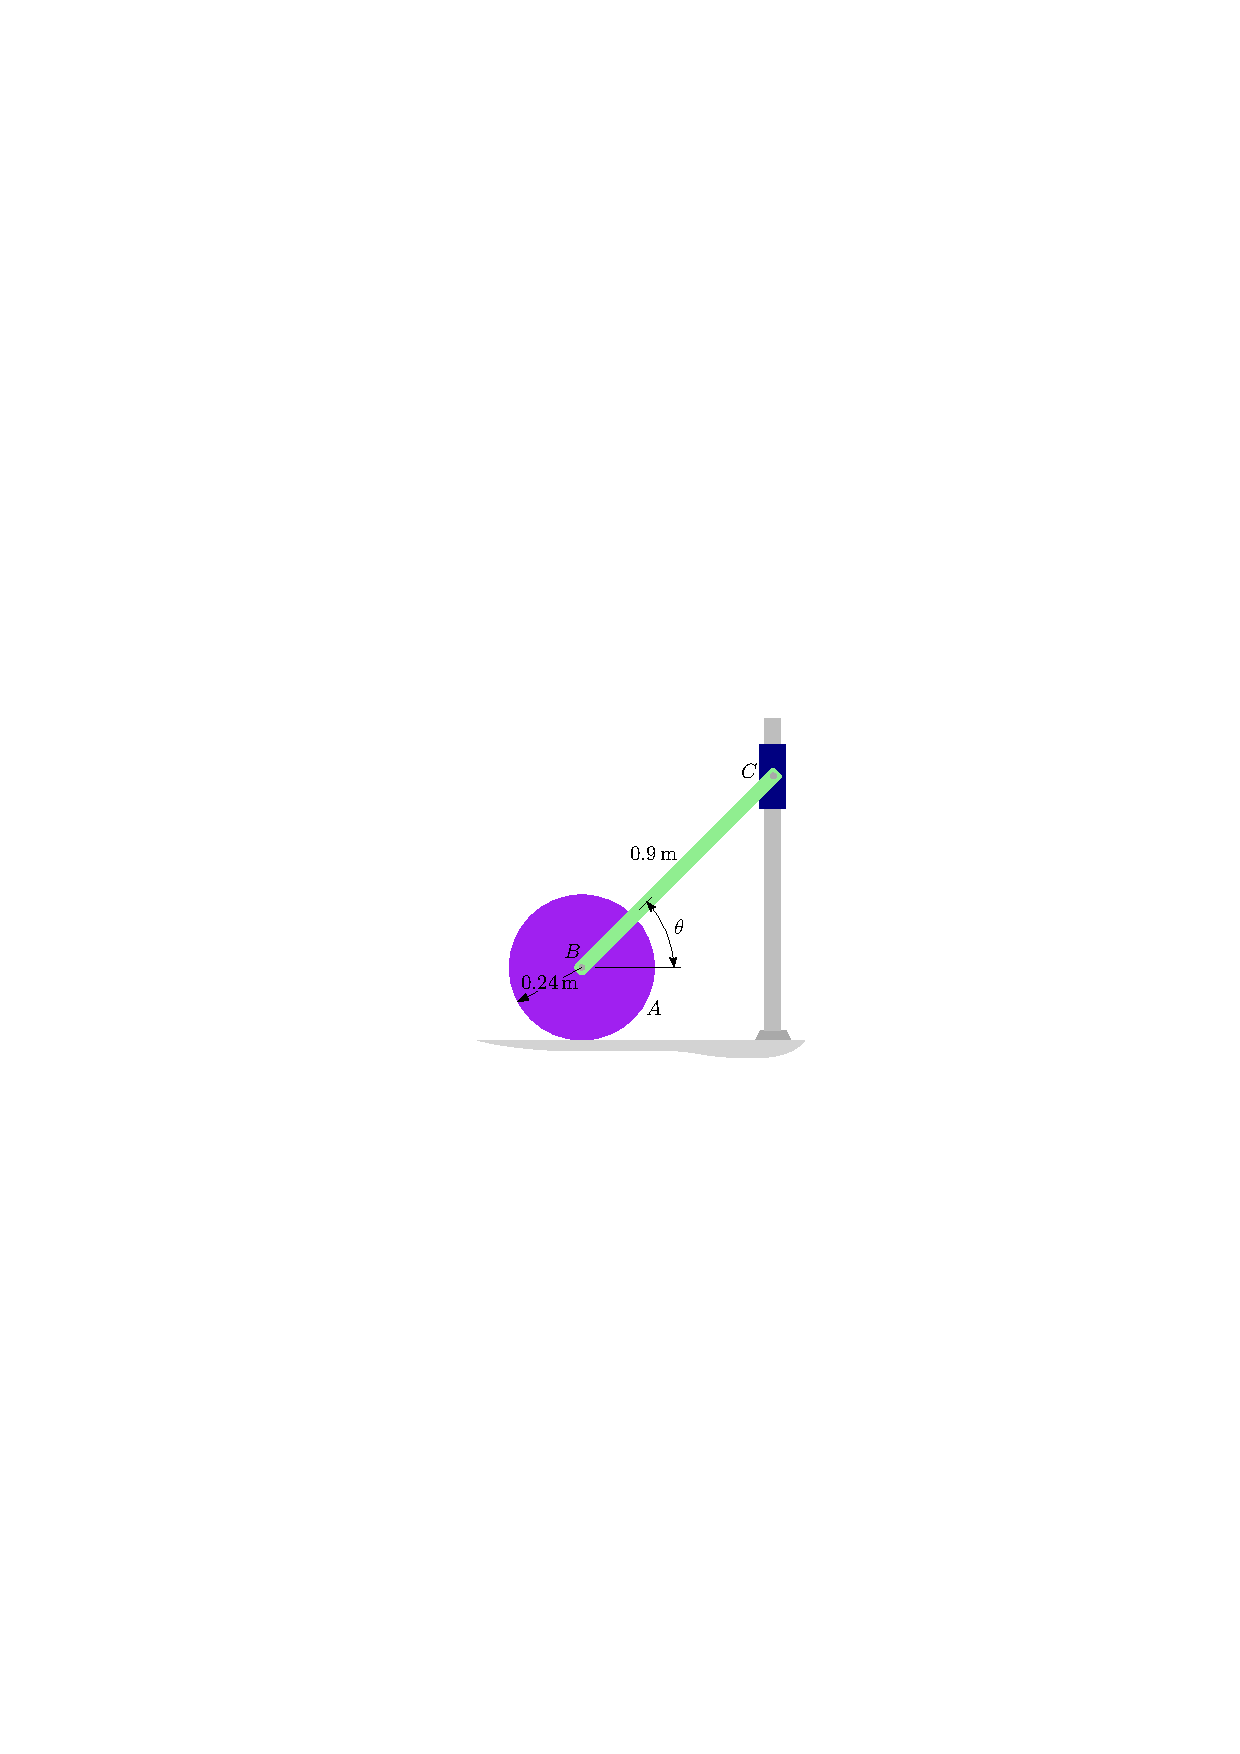
\includegraphics[scale=1.2]{../../images/draw_6}
\end{flushright}